The purpose of this case is to test the loss ratio sampling when the lognormal vulnerability model has nonzero coefficients of variation of the loss ratios. Table~\ref{tab:vf-ln-tax1-nzcov} shows the mean loss ratios and corresponding coefficients of variation in the vulnerability model used in this test case.

Apart from the nonzero coefficients of variation in the vulnerability model, this case is similar to Case~1a. The only difference enters during the loss ratio sampling stage, where the lognormal distribution no longer devolves into the degenerate distribution.

As in Case~1a, the mean loss ratio and coefficient of variation of the loss ratio are obtained by linear interpolation from the provided vulnerability model for each of the 4,115 ground motion values produced by the hazard calculation. A loss ratio is now sampled from the lognormal distribution defined by the interpolated mean and standard deviation parameters for each ground motion value. The rest of the calculation steps involved in the computation of the event loss table, loss exceedance curve, and average annual loss remain the same as described in Case~1a.

The loss curve calculated using the implementation of the calculator in Julia is compared with that produced by OpenQuake in Figure~\ref{fig:lc-ebr-1d}.

\begin{figure}[htbp]
\centering
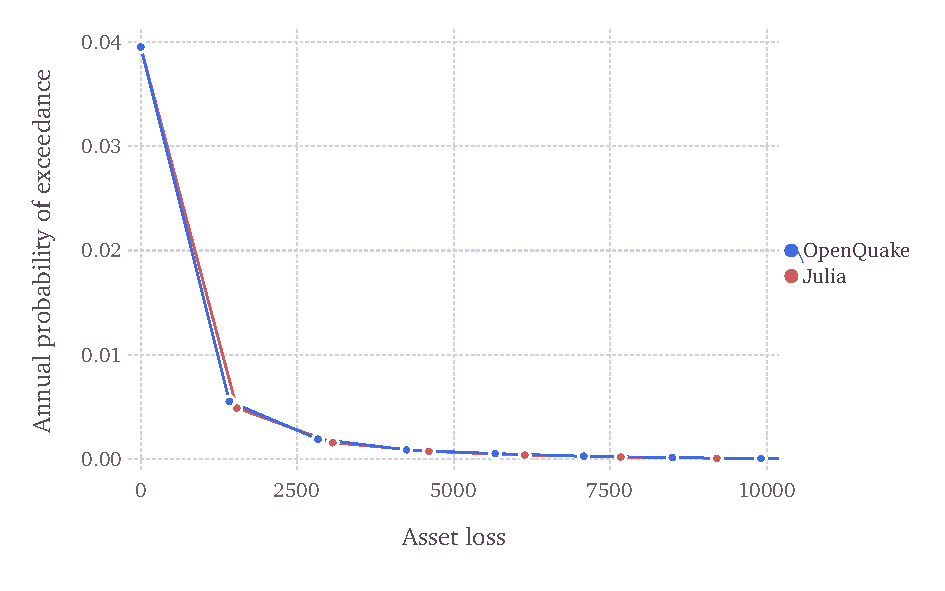
\includegraphics[width=12cm]{qareport/figures/fig-lc-ebr-1d}
\caption{Loss curve comparison for event based risk test case 1d}
\label{fig:lc-ebr-1d}
\end{figure}

The area under the annual loss exceedance curve gives the average annual loss.